	\begin{multicols}{3}
		\begin{minipage}{.3\paperheight}
			\maketitle
			\tableofcontents
		\end{minipage}
		\section{Grundlagen}
		\subsection{Mathematik}
		%\begin{tabularx}{.5\textwidth}{c|X|X|X|}
		%	& Kartesische Koordinaten & Zylindrische Koordinaten & Kugel-Koordinaten\\
		%	Kartesisch & \(\begin{pmatrix} x\\ y\\ z\end{pmatrix}\) & \(\begin{pmatrix}q\end{pmatrix}\) & \(\begin{pmatrix}q\end{pmatrix}\) \\
		%	Zylindrisch & \(\begin{pmatrix}q\end{pmatrix}\) & \(\begin{pmatrix} \rho\\ \varphi\\ z\end{pmatrix}\) &  \(\begin{pmatrix}q\end{pmatrix}\) \\
		%	Kugel & \(\begin{pmatrix}q\end{pmatrix}\) & \(\begin{pmatrix}q\end{pmatrix}\) & \(\begin{pmatrix} r\\ \theta\\ \varphi\end{pmatrix}\)% 
		%\end{tabularx}
	 \subsection{Maxwell-Gleichungen}
	 \subsubsection{Integralform}
{\small%
\begin{flalign*}
& \mathrm{\textbf{Gauß'sche Gesetz:}}\\
& \iint\limits_{A(V)}\vec{D}_m\cdot\mathrm{d}\vec{A} = \iiint\limits_V\rho\mathrm{d}V = Q\\
& \mathrm{\textbf{Magnetische Quellenfreiheit:}}\\
& \iint\limits_{A(V)}\vec{b}\cdot\mathrm{d}\vec{A} = 0\\
 & \mathrm{\textbf{Induktionsgesetz:}}\\
 & \oint\limits_C\vec{e}\cdot\mathrm{d}\vec{s} =%
 -\dfrac{\mathrm{d}}{\mathrm{d}\vec{t}}\iint\limits_A\vec{b}\cdot\mathrm{d}\vec{A} = -\dfrac{\mathrm{d}\Phi_m}{\mathrm{d}t}\\
 & \mathrm{\textbf{Durchflutungsgesetz:}}\\
 & \oint\limits_C\vec{h}\cdot\mathrm{d}\vec{s} = \iint\limits_A\left[\vec{j}+\dfrac{\mathrm{d}\vec{D}_m}{\mathrm{d}t}\right]\cdot\mathrm{d}\vec{A} = i_{ges}\\
 \end{flalign*}
}
	 \subsubsection{(Zeitfreie) Differentielle Form}
	 {\small%
	 \begin{align*}
	  &\mathrm{\textbf{Differentiell}} & \mathrm{\textbf{Zeitfrei (harm. Wellen)}}\\
	 	&\nabla\times\vec{e} = -\dfrac{\partial\vec{b}}{\vec{\partial t}} & \nabla\times\vec{E} = -j\omega\vec{B}\\
	 	&\nabla\times\vec{h} = \vec{j} +\dfrac{\partial\vec{D}_m}{\vec{\partial t}} & \nabla\times\vec{H} = \vec{J} + j\omega\vec{D}_m\\
		&\nabla\cdot\vec{D}_m = \rho & \nabla\cdot\vec{D}_m = \rho\\
		&\nabla\cdot\vec{b} = \rho_m & \nabla\cdot\vec{B} = \rho_m
	 \end{align*}
	 }
	 \subsubsection{Kontinuitätsgleichung des Stroms}
	 {\small%
	 \begin{flalign*}
	 	& \mathrm{\textbf{Integrale Form}}\\
		& \oint\limits_{A(V)}\vec{j}\cdot\mathrm{d}\vec{A} = -\int\limits_v \dfrac{\partial \rho}{\partial t} \mathrm{d}v\\
		& \mathrm{\textbf{Differentielle Form}}\\
		& \nabla\cdot\vec{j} = -\dfrac{\partial \rho}{\partial t}\\
		& \mathrm{\textbf{Zeitfreie Form}}\\
		& \nabla\cdot\vec{J} = -j\omega\rho
	 \end{flalign*}
	 \subsubsection{Entkopplung der Maxwell-Gleichungen}
	 \begin{itemize}
	 	\itemsep0pt
		\item Differentielle Maxwell-Gleichungen
		\item \(\epsilon_r, \mu_r = \mathrm{konst.}\)
		\item \(\kappa = 0, \vec{J} \neq 0\)\\
	 	\(\implies\) \textbf{Wellengleichung:}\\\vspace{2pt}
		\(\nabla\!\times\!\nabla\!\times\!\vec{E} - k^2\vec{E} = -j\omega\mu_r\mu_0\vec{J}\)
		\item Quellenfrei \(\vec{J} = 0\)
		\item \(\nabla\!\times\!\nabla\!\times\!\vec{F} = \mathrm{grad}\;\mathrm{div}\vec{F} - \Delta\vec{F}\)\\
		\(\implies\) \textbf{Helmholtz-Gleichung:} \(\Delta\vec{E} + k^2\vec{E} = 0\)
	 \end{itemize}
	 
	 \subsubsection{Rand- und Stetigkeitsbedingungen}
	 \begin{itemize}
	 	\itemsep0pt
		\item \textbf{Tangentialkomponenten}
		\begin{itemize}
			\itemsep0pt
			\item Normalfall: \(\vec{n}\times\left(\vec{h}_1 - \vec{h}_2\right) = 0\)
			\item Oberflächenströme: \(\vec{n}\times\left(\vec{h}_1 - \vec{h}_2\right) = \vec{j}_F\)
			\item \(\vec{n}\times\left(\vec{e}_1 - \vec{e}_2\right) = 0\)
		\end{itemize}
		\item \textbf{Normalkomponenten}
		\begin{itemize}
			\itemsep0pt
			\item Normalfall: \(\vec{n}\cdot\left(\vec{D}_{m1} - \vec{D}_{m2}\right) = 0\)
			\item Oberflächenladungen: \(\vec{n}\cdot\left(\vec{D}_{m1} - \vec{D}_{m2}\right) = \rho_F\)
			\item \(\vec{n}\cdot\left(\vec{b}_1 - \vec{b}_2\right) = 0\)
		\end{itemize}
	 \end{itemize}
	 }
	 
	 \subsection{Skin-Effekt}%
	 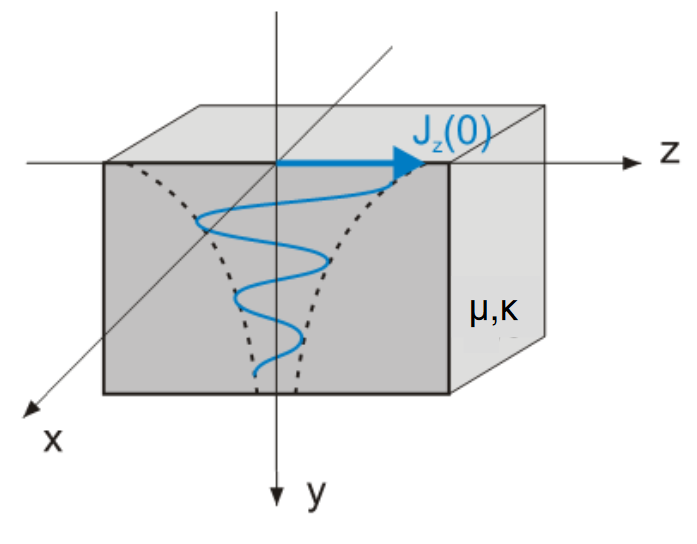
\includegraphics[width=.3\paperheight]{content/fuw/pictures/skin_effect.png}
	 {\small%
	 \begin{itemize}
	 	\itemsep0pt
		\item ideale Leiter \(\kappa\to\infty:\: E_{tan} = 0\)\\
		\(\implies\) nur in einer infitesimal dünnen Schicht existieren Oberflächenströme
		\item guter Leiter \(\kappa\gg\omega\epsilon\), verlustbehaftet:\\
		\(\implies\) in einer dünnen Schicht unter der Oberfläche existieren nennenswerte Stromdichten\\
		\(\implies\) Für die Verluste sind nur die obersten Schichten des Leiters entscheidend
	 \end{itemize}
	 }
	 \subsection{Ebene Wellen}
	 \subsection{Reflexion und Brechung}
	 \subsection{Gauß'scher Strahl}
	 \subsection{TEM-Leitungen}
	 \subsection{Planare Leitungen}
	\end{multicols}
